\begin{figure}[bth!]
  \begin{center}
    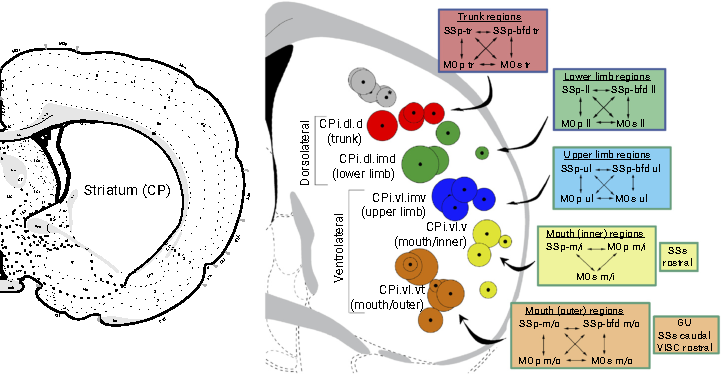
\includegraphics[width=0.9\linewidth]{ch-intro/figures/StriatumInputMap}
    \caption[Somatotopic map of cortical inputs to \gls{dls}]
    {\textbf{Somatotopic map of cortical inputs to \gls{dls}.}
    \textit{Left}: striatum in the rat brain atlas.
    \textit{Right}: input from somatosensory cortices form a topographic map in the \gls{dls}.
    Abbreviations are defined in the original reference and are not important for the purposes of this work.
    Figure adopted from~\cite{Hintiryan2016NN}.
    }
    \label{fig:intro:InputMap}
  \end{center}
\end{figure}